\documentclass{beamer}

\usepackage[slovene]{babel}
\usepackage{amsfonts,amssymb}
\usepackage[utf8]{inputenc}
\usepackage{lmodern}
\usepackage[T1]{fontenc}
\usepackage{graphics}

\usetheme{CambridgeUS}

\makeatletter
\setbeamertemplate{footline}
{
  \leavevmode%
  \hbox{%
  \begin{beamercolorbox}[wd=.333333\paperwidth,ht=2.25ex,dp=1ex,center]{author in head/foot}%
    \usebeamerfont{author in head/foot}\insertshortauthor%~~\beamer@ifempty{\insertshortinstitute}{}{(\insertshortinstitute)}
  \end{beamercolorbox}%
  \begin{beamercolorbox}[wd=.333333\paperwidth,ht=2.25ex,dp=1ex,center]{title in head/foot}%
    \usebeamerfont{title in head/foot}\insertshorttitle
  \end{beamercolorbox}%
  \begin{beamercolorbox}[wd=.333333\paperwidth,ht=2.25ex,dp=1ex,right]{date in head/foot}%
    \usebeamerfont{date in head/foot}\insertshortdate{}\hspace*{2em}
    \insertframenumber{} / \inserttotalframenumber\hspace*{2ex} 
  \end{beamercolorbox}}%
  \vskip0pt%
}
\makeatother

\def\N{\mathbb{N}} % mnozica naravnih stevil
\def\Z{\mathbb{Z}} % mnozica celih stevil
\def\Q{\mathbb{Q}} % mnozica racionalnih stevil
\def\R{\mathbb{R}} % mnozica realnih stevil
\def\C{\mathbb{C}} % mnozica kompleksnih stevil


\def\qed{$\hfill\Box$}   % konec dokaza
\newtheorem{izrek}{Izrek}
\newtheorem{trditev}{Trditev}
\newtheorem{posledica}{Posledica}
\newtheorem{lema}{Lema}
\newtheorem{definicija}{Definicija}
\newtheorem{pripomba}{Pripomba}
\newtheorem{primer}{Primer}
\newtheorem{zgled}{Zgled}
\newtheorem{zgledi}{Zgledi uporabe}
\newtheorem{rešitev}{Rešitev}
\newtheorem{ideja}{Ideja}
\newtheorem{pr}{Naloga}

\title{Škatlasti zlepki}
\author[Sandra Kerševan, Sara Močnik]{Sandra Kerševan in Sara Močnik}
\institute{Fakulteta za matematiko in fiziko \\
Oddelek za matematiko}
\date{januar 2021}


\begin{document}


%%%%%%%%%%%%%%%%%%%%%%%%%%%%%%%%%%%%%%%%%%%%%%%%%%%%%%%%%%%

\begin{frame}
\titlepage
\end{frame}

%%%%%%%%%%%%%%%%%%%%%%%%%%%%%%%%%%%%%%%%%%%%%%%%%%%%%%%%%%%

\begin{frame}

\frametitle{Motivacija}

Škatlasti zlepek:
\begin{itemize}
\item zlepki polinomskih funkcij več spremenljivk
\item uporabni pri aproksimaciji in interpolaciji funkcije več spremenljivk
\end{itemize}

\begin{figure}
    \centering
    \includegraphics[scale=0.3]{boxsplines}
    \caption{Škatlasti zlepki dveh spremenljivk v prostoru z 1, 2, 3 in 4 vektorji.}
\end{figure}

\end{frame}

%%%%%%%%%%%%%%%%%%%%%%%%%%%%%%%%%%%%%%%%%%%%%%%%%%%%%%%%%%%

\begin{frame}

\frametitle{Škatlasti zlepki tipa 1 \\ Triangulacija}

Regularna triangulacija tipa 1: 

\begin{figure}
    \centering
    \includegraphics[scale=0.23]{triangulacija1}
    \caption{Regularna triangulacija tipa 1.}
\end{figure}


Oznaka: $\Delta_I$ \\
Točke triangulacije: $(x,y) = v \in \mathbb{Z} \times \mathbb{Z}$


\end{frame}

%%%%%%%%%%%%%%%%%%%%%%%%%%%%%%%%%%%%%%%%%%%%%%%%%%%%%%%%%%%%%%%%%%%%%

\begin{frame}
\frametitle{Škatlasti zlepki tipa 1}

\begin{definicija}
Prostor $C^r$ zlepkov stopnje n: $S_d^r(\Delta_I) = \{ s \in C^r(\Omega):\ s|_T \in \mathbb{P}_d^2\  \forall T \in  \Delta_I\}$
\end{definicija}

\vspace{5mm}
Cilj: \\
Konstruirati zlepke $B$, $B \in S_n^r (\Delta_I)$, za katere velja:
\begin{enumerate}
\item Nosilec zlepka B je majhen.  $\big[ supp\ B = nosilec\ B = \overline{\{x;\ Bx \neq 0\}}\ \big] $
\item B je pozitiven na $Int(supp\ B)$.
\item $S := Lin \{ B(v-\mu)  \}_{\mu \in \mathbb{Z}^2}$ vsebuje polinome stopnje $d$.
\item $\sum_{\mu \in \mathbb{Z}^2} B(v-\mu)  = 1$ za vse $v \in \mathbb{R}^2$
\item Prostor $S$ aproksimira gladke funkcije na poljubni kompaktni podmnožici $\mathbb{R}^2$.
\end{enumerate}

\end{frame}

%%%%%%%%%%%%%%%%%%%%%%%%%%%%%%%%%%%%%%%%%%%%%%%%%%%%%%%%%%%

\begin{frame}
\frametitle{Škatlasti zlepki tipa 1 \\ Smeri triangulacije}

Smeri v triangulaciji:
\begin{itemize}
\item premik v levo: $e_1 = (1,0)$
\item premik navzgor: $e_2 = (0,1)$
\item premik po diagonali: $e_3 = (1,1)$
\end{itemize}

\vspace{5mm}

Za $n \geq 3$ definiramo množico  $$X_n := \{v_1, v_2, \ldots , v_n\},$$ kjer so $v_i \in \{e_1, e_2, e_3\}$ in $X_n$ vsebuje vsako od smeri $e_1, e_2, e_3$ vsaj enkrat. \\
Množici $X_n$ rečemo \textbf{množica smeri tipa 1}.\\
\vspace{4mm}
$X_3 = \{e_1,e_2, e_3\}$
\end{frame}

%%%%%%%%%%%%%%%%%%%%%%%%%%%%%%%%%%%%%%%%%%%%%%%%%%%%%%%%%%%

\begin{frame}
\frametitle{Škatlasti zlepki tipa 1 \\ Najmanjši zlepek}

$$B_{111} \in S_1^0(\Delta_I)$$
$$B_{111} ((1,1)) = 1$$
$$B_{111} (v) = 0\ \forall v \neq (1,1)$$

\begin{figure}
    \centering
    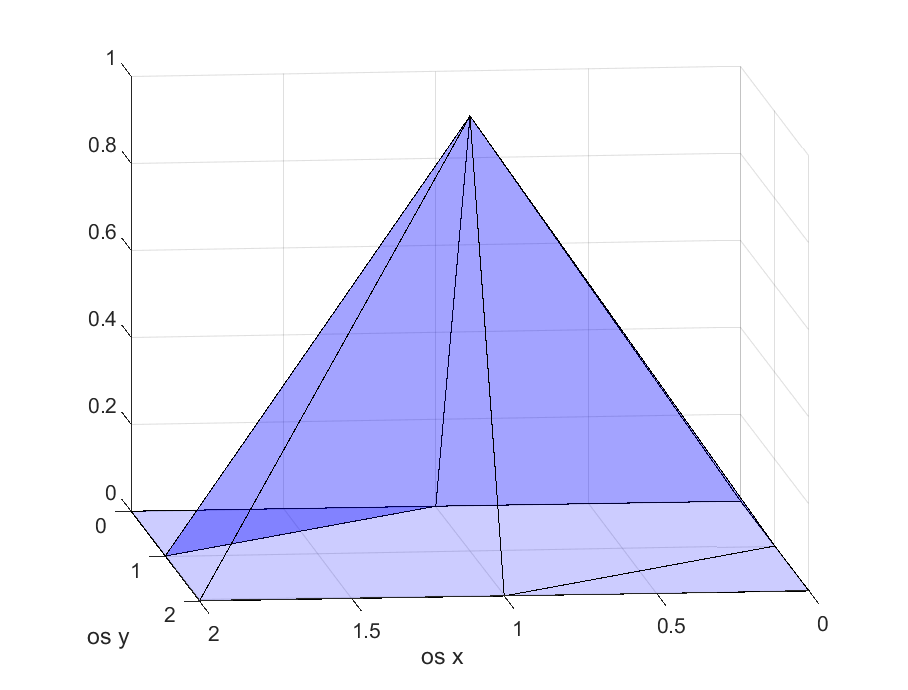
\includegraphics[scale=0.23]{B111}
    \caption{Zlepek $B_{111}$.}
\end{figure}
\end{frame}

%%%%%%%%%%%%%%%%%%%%%%%%%%%%%%%%%%%%%%%%%%%%%%%%%%%%%%%%%%%%%%%%%%%%%

\begin{frame}
\frametitle{Škatlasti zlepki tipa 1 \\ Zlepki višjih stopenj}

\begin{definicija}
Naj bo $n > 3$ in $X_n := \{v_1, v_2, \ldots , v_n\}$ množica smeri tipa 1.
Definirajmo množice $X_i := \{v_1, v_2, \ldots , v_i\}$ za $i = 3, 4, \ldots, n$.
Potem za $4 \leq i \leq n$ rekurzivno definiramo škatlati zlepek tipa 1  z enačbo:
$$B(v|X_i) := \int_0^1 B(v-tv_i | X_{i-1}) dt,$$
kjer je $B(v|X_3)$ škatlasti zlepek $B_{111}$.
\end{definicija}

\vspace{5mm}

Oznaka: \\
\textbf{$B_{ijk}(v)$} škatlasti zlepek tipa 1 $B(v|X_n)$, kjer je $X_n$ množica smeri tipa 1, za katero velja: $X_n = \{e_1^{<i>},e_2^{<j>}, e_3^{<k>}\}$.

\end{frame}

%%%%%%%%%%%%%%%%%%%%%%%%%%%%%%%%%%%%%%%%%%%%%%%%%%%%%%%%%%%

\begin{frame}
\frametitle{Škatlasti zlepki tipa 1}

\begin{izrek}
Naj bo $X_n$ množica smeri tipa 1.\\
Škatlasti zlepek $B(v|X_n)$ ima nosilec na zaprtju množice
$$[X_n] := \{ \sum_{j=1}^n t_j v_j : \ 0 \leq t_j < 1; \ j = 1, \ldots, n\}$$.
Za vse točke $v$ v notranjosti množice $[X_n]$ je $B(v|X_n) > 0$.
\end{izrek}

\vspace{5mm}

Množici $[X_n]$ rečemo tudi afina kocka $X_n$.
\end{frame}

%%%%%%%%%%%%%%%%%%%%%%%%%%%%%%%%%%%%%%%%%%%%%%%%%%%%%%%%%%%%%%%%%%%%%

\begin{frame}
\frametitle{Škatlasti zlepki tipa 1}

\begin{figure}
    \centering
    \includegraphics[scale=0.32]{nosilci}
    \caption{Nosilci za $B_{111}$, $B_{211}$, $B_{222}$ in $B_{322}$.}
\end{figure}

\end{frame}

%%%%%%%%%%%%%%%%%%%%%%%%%%%%%%%%%%%%%%%%%%%%%%%%%%%%%%%%%%%%%%%%%%%%%

\begin{frame}
\frametitle{Škatlasti zlepki tipa 1 \\ Odvodi}

Dan imamo vektor $u = (u_1, u_2) \in \mathbb{R}^2$, $u \neq (0,0)$. \\
Naj bo $D_u$ smerni odvod, %???? 
$ \bigtriangledown_u$ pa nazaj diferenčen operator, %????
za katerega velja:
$$\bigtriangledown_u f(\cdot) = f(\cdot) - f(\cdot - u)$$.

\vspace{5mm}

\begin{lema}
\label{lema1}
Naj bo $X_n$ množica smeri tipa 1 in naj bo $n\geq 4$.\\
Potem za $4 \leq j < n$ velja:
$$D_{v_j} B(\cdot|X_n) = \bigtriangledown_{v_j} B(\cdot | X_n \setminus \{v_j\}).$$
\end{lema}
\end{frame}
%%%%%%%%%%%%%%%%%%%%%%%%%%%%%%%%%%%%%%%%%%%%%%%%%%%%%%%%%%%%%%%%%%%%%

\begin{frame}
\frametitle{Škatlasti zlepki tipa 1}

\begin{izrek}
Naj bo $X_n = \{e_1^{<i>},e_2^{<j>}, e_3^{<k>}\}$ množica smeri tipa 1 in $i+j+k = n$.
Potem $B_{ijk} := B(\cdot | X_n) \in S_{n-2}^r (\Delta_I)$, kjer je $$r := r(X_n) = min\{i+j, j+k, k+i\} -2.$$
\end{izrek}

\vspace{3mm}
\pause

Zgornji izrek nam da naslednje rezultate:
\begin{itemize}
\item $B_{111} := B(\cdot | X_3) \in S_{1}^0 (\Delta_I)$
\item $B_{221} := B(\cdot | X_5) \in S_{3}^1 (\Delta_I)$
\item $B_{222} := B(\cdot | X_6) \in S_{4}^2 (\Delta_I)$
\item $B_{322} := B(\cdot | X_7) \in S_{5}^2 (\Delta_I)$
\item $B_{332} := B(\cdot | X_8) \in S_{6}^3 (\Delta_I)$
\item $B_{333} := B(\cdot | X_9) \in S_{7}^4 (\Delta_I)$
\end{itemize}

\end{frame}
%%%%%%%%%%%%%%%%%%%%%%%%%%%%%%%%%%%%%%%%%%%%%%%%%%%%%%%%%%%%%%%%%%%%%

\begin{frame}
\frametitle{Škatlasti zlepki tipa 1 \\ B-ordinate}

$X_n := \{v_1, v_2, \ldots , v_n\}$ je množica smeri tipa 1. Zanjo velja, da je $v_i \in \{e_1, e_2, e_3\}$ .

Potem je $D_{v_i} B(v|X_n)$ na kateremkoli trikotniku triangulacije smerni odvod v smeri ene od stranic trikotnika. 

Po lemi od prej velja: $$D_{v_j} B(v|X_n) = \bigtriangledown_{v_j} B(v | X_n \setminus \{v_j\}).$$
\end{frame}

%%%%%%%%%%%%%%%%%%%%%%%%%%%%%%%%%%%%%%%%%%%%%%%%%%%%%%%%%%%%%%%%%%%%%

\begin{frame}
\frametitle{Škatlasti zlepki tipa 1 \\ B-ordinate}

$$p_{n-2} (v) := \sum_{i+j+k=n-2} c_{ijk} B_{ijk}^{n-2}(v)$$
Oznaka za zožitev $B(\cdot | X_n)$ na trikotnik $T = \langle (0,0), (1, 0), (1,1)\rangle$.\\
Vemo: $B_{ijk}^{n-2}(v) = \frac{(n-2)!}{i! j! k!} u^i v^j w^k$, $i, j, k \in \mathbb{N}_0, i+j+k=n-2$ in $(u,v, w ) = Bar(v; T)$

Potem velja:
$$D_{e_1} p_{n-2} (v) = (n-2)\sum_{i+j+k=n-3} (c_{i,j+1,k} - c_{i+1, j, k}) B_{ijk}^{n-3}(v)$$
$$D_{e_2} p_{n-2} (v) = (n-2)\sum_{i+j+k=n-3} (c_{i,j,k+1} - c_{i, j+1, k}) B_{ijk}^{n-3}(v)$$
$$D_{e_3} p_{n-2} (v) = (n-2)\sum_{i+j+k=n-3} (c_{i,j,k+1} - c_{i+1, j, k}) B_{ijk}^{n-3}(v)$$

\end{frame}


%%%%%%%%%%%%%%%%%%%%%%%%%%%%%%%%%%%%%%%%%%%%%%%%%%%%%%%%%%%%%%%%%%%%%

\begin{frame}
\frametitle{Škatlasti zlepki tipa 2 \\ Triangulacija}

Regularna triangulacija tipa 2: 

\begin{figure}
    \centering
    \includegraphics[scale=0.23]{triangulacija2}
    \caption{Regularna triangulacija tipa 2.}
\end{figure}


Oznaka: $\Delta_{II}$ \\

\end{frame}
%%%%%%%%%%%%%%%%%%%%%%%%%%%%%%%%%%%%%%%%%%%%%%%%%%%%%%%%%%%%%%%%%%%%%

\begin{frame}
\frametitle{Škatlasti zlepki tipa 2}

Smeri v triangulaciji:
\begin{itemize}
\item premik v levo: $e_1 = (1,0)$
\item premik navzgor: $e_2 = (0,1)$
\item premik po diagonali: $e_3 = (1,1)$
\item premik po drugi diagonali: $e_3 = (-1,1)$
\end{itemize}

\vspace{5mm}

Za $n \geq 3$ definiramo množico  $$X_n := \{v_1, v_2, \ldots , v_n\},$$ kjer so $v_i \in \{e_1, e_2, e_3, e_4\}$ in $X_n$ vsebuje vsako od smeri $e_1, e_2, e_3, e_4$ vsaj enkrat. \\
Množici $X_n$ rečemo \textbf{množica smeri tipa 2}.\\
\vspace{4mm}
$X_4 = \{e_1,e_2, e_3, e_4\}$

\end{frame}
%%%%%%%%%%%%%%%%%%%%%%%%%%%%%%%%%%%%%%%%%%%%%%%%%%%%%%%%%%%%%%%%%%%%%

\begin{frame}
\frametitle{Škatlasti zlepki tipa 2 \\ Najmanjši zlepek}

$$B_{1111} \in S_2^1(\Delta_{II})$$



\begin{figure}
    \centering
    \begin{minipage}{0.45\textwidth}
        \centering
        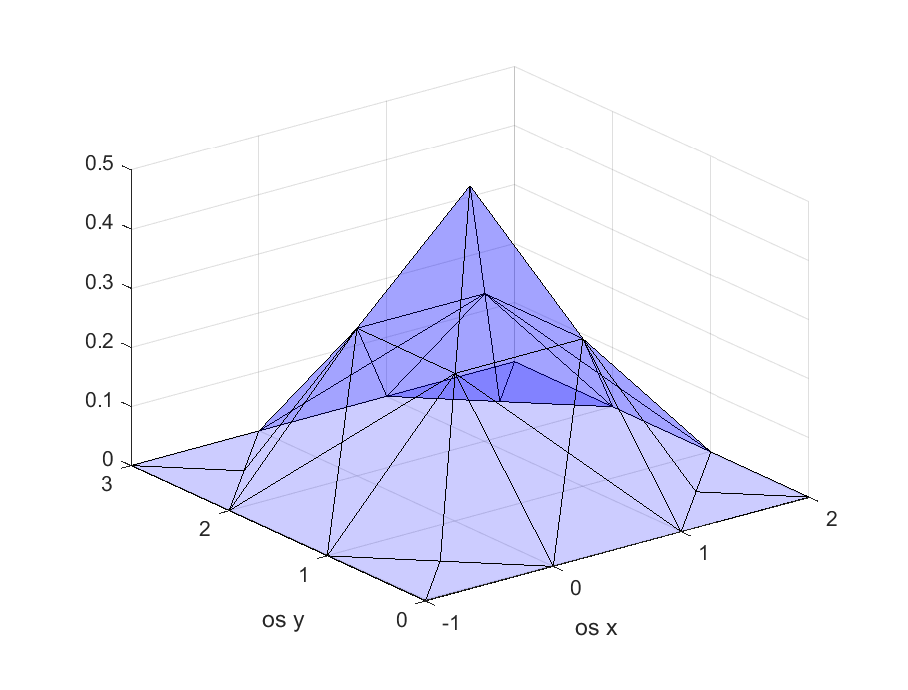
\includegraphics[width=1\textwidth]{B1111} % first figure itself
        \caption{Zlepek $B_{1111}$.}
    \end{minipage}\hfill
    \begin{minipage}{0.45\textwidth}
        \centering
        \includegraphics[width=0.7\textwidth]{B1111a} % second figure itself
        \caption{B-ordinate $16 B_{1111}$.}
    \end{minipage}
\end{figure}

\end{frame}


%%%%%%%%%%%%%%%%%%%%%%%%%%%%%%%%%%%%%%%%%%%%%%%%%%%%%%%%%%%%%%%%%%%%%

\begin{frame}
\frametitle{Škatlasti zlepki tipa 2 \\ Zlepki višjih stopenj}

\begin{definicija}
Naj bo $n > 4$ in $X_n := \{v_1, v_2, \ldots , v_n\}$ množica smeri tipa 2.
Definirajmo množice $X_i := \{v_1, v_2, \ldots , v_i\}$ za $i = 4, \ldots, n$.
Potem za $5 \leq i \leq n$ rekurzivno definiramo škatlati zlepek tipa 2  z enačbo:
$$B(v|X_i) := \int_0^1 B(v-tv_i | X_{i-1}) dt,$$
kjer je $B(v|X_4)$ škatlasti zlepek $B_{1111}$.
\end{definicija}

\vspace{5mm}

Oznaka: \\
\textbf{$B_{ijkl}(v)$} škatlasti zlepek tipa 1 $B(v|X_n)$, kjer je $X_n$ množica smeri tipa 2, za katero velja: $X_n = \{e_1^{<i>},e_2^{<j>}, e_3^{<k>}, e_4^{<l>}\}$.

\end{frame}


%%%%%%%%%%%%%%%%%%%%%%%%%%%%%%%%%%%%%%%%%%%%%%%%%%%%%%%%%%%

\begin{frame}
\frametitle{Škatlasti zlepki tipa 2}

\begin{izrek}
Naj bo $X_n = \{e_1^{<i>},e_2^{<j>}, e_3^{<k>}, e_4^{<l>}\}$ množica smeri tipa 2 in $i+j+k+l = n$.
Potem $B_{ijkl} := B(\cdot | X_n) \in S_{n-2}^r (\Delta_{II})$, kjer je $r := r(X_n) = min\{i+k+l, j+k+l, i+j+k, i+j+l\} -2$.
\end{izrek}

\vspace{3mm}
\pause

Zgornji izrek nam da naslednje rezultate:
\begin{itemize}
\item $B_{1111} := B(\cdot | X_4) \in S_{2}^1 (\Delta_{II})$
\item $B_{2111} := B(\cdot | X_5) \in S_{3}^1 (\Delta_{II})$
\item $B_{2211} := B(\cdot | X_6) \in S_{4}^2 (\Delta_{II})$
\item $B_{2221} := B(\cdot | X_7) \in S_{5}^3 (\Delta_{II})$
\item $B_{2222} := B(\cdot | X_8) \in S_{6}^2 (\Delta_{II})$
\end{itemize}

\end{frame}
%%%%%%%%%%%%%%%%%%%%%%%%%%%%%%%%%%%%%%%%%%%%%%%%%%%%%%%%%%%%%%%%%%%%%


\begin{frame}

\frametitle{Vrsta iz škatlastega zlepka}

Opazujemo vrste tipa: $$s(\cdot) := \sum_{j\in\Z^2} c_j B(\cdot - j | X_n) $$

Linearni prostor škatlastih zlepkov: $$S(X_n) := \{ \sum_{j\in\Z^2} c_j B(\cdot - j | X_n) ; c_j \in \R\, \text{za}\, \forall j\in\Z^2 \}$$


\end{frame}

%%%%%%%%%%%%%%%%%%%%%%%%%%%%%%%%%%%%%%%%%%%%%%%%%%%%%%%%%%%

\begin{frame}

\frametitle{}

\begin{izrek}
	Naj bo $X_n$ množica smeri tipa 1 ali 2. Potem pripadajoči škatlasti zlepki tvorijo particijo enote na $\R^2$ oz. velja $$ \sum_{j\in\Z^2} B(\cdot - j | X_n) = 1. $$
\end{izrek}

\vspace{3mm}
\pause

\begin{izrek}
	Naj bo $X_n$ množica smeri tipa 2. Potem velja $$ \sum_{(j_1,j_2)\in\Z^2} B(\cdot - j_1 e_3 - j_2 e_4 | X_n) = \frac{1}{2}. $$
\end{izrek}


\end{frame}

%%%%%%%%%%%%%%%%%%%%%%%%%%%%%%%%%%%%%%%%%%%%%%%%%%%%%%%%%%%%%%%%%%%%%

\begin{frame}

\frametitle{Linearna neodvisnost}

Premaknjeni škatlasti zlepki $\{B(\cdot - j | X_n)\}_{j\in\Z^2}$ so \textbf{linearno neodvisni}, kadar velja: $$\sum_{j\in\Z^2} a_j B(v - j | X_n) = 0 \, \text{za} \, \forall v\in\R^2 \implies a_j = 0 \, \text{za} \, \forall j\in\Z^2.$$

\end{frame}

%%%%%%%%%%%%%%%%%%%%%%%%%%%%%%%%%%%%%%%%%%%%%%%%%%%%%%%%%%%%%%%%%%%%%

\begin{frame}

\frametitle{Linearna neodvisnost}

\begin{izrek}
	Naj bo $X_n$ množica smeri tipa 1. Potem je množica $\{B(\cdot - j | X_n)\}_{j\in\Z^2}$ linearno neodvisna.
	
	Velja tudi: Naj bo $a = \{a_j\}_{j\in\Z^2}$ omejeno zaporedje. Potem velja $$A \left\lVert a \right\rVert_\infty \leq \left\lVert \sum_{j\in\Z^2} a_j B(\cdot - j | X_n) \right\rVert_\infty \leq \left\lVert a \right\rVert_\infty,$$ kjer je $\left\lVert a \right\rVert_\infty = \max_{j\in\Z^2}|a_j|.$
\end{izrek}

\pause

\begin{izrek}
	Naj bo $X_n$ množica smeri tipa 2. Potem je množica $\{B(\cdot - j | X_n)\}_{j\in\Z^2}$ linearno odvisna.
\end{izrek}

\end{frame}

\end{document}